\documentclass[12pt]{article}
\usepackage[margin=1in]{geometry}
\usepackage{times}
\usepackage{parskip}
\usepackage{titlesec}
\usepackage{graphicx}
\usepackage{float}
\usepackage{hyperref}
\usepackage{cite}
\usepackage{tikz}
\usetikzlibrary{shapes.geometric, arrows.meta, positioning, calc}

% ---- Section formatting ----
\titleformat{\section}{\large\bfseries}{{\thesection.}}{0.5em}{}
\titleformat{\subsection}{\normalsize\bfseries}{{\thesubsection}}{0.5em}{}
\titleformat{\subsubsection}{\normalsize\bfseries}{{\thesubsubsection}}{0.5em}{}

\begin{document}

% ========== Title Page ==========
\begin{center}
\vspace*{2cm}
{\LARGE \textbf{ButterFlight}}\\[0.4cm]
{\large Maya Plug-in Design Document}\\[3cm]
{\large By: Cecilia Chen and Yiding Tian}\\[4cm]
{\large Based on:}\\[0.3cm]
{\normalsize A Practical Model for Realistic Butterfly Flight Simulation.}\\[0.2cm]
{\normalsize Chen, Q., Lu, T., Tong, Y., Luo, G., Jin, X., and Deng, Z., 2022.}\\
{\normalsize ACM Transactions on Graphics (TOG).}\\[3cm]
{\large CIS 6600 --- Advanced Topics in Computer Graphics and Animation}\\[0.3cm]
{\large Instructor: Dr.~Stephen Lane}
\end{center}

\newpage

% ========== Project Summary ==========
\section*{Project Summary}

Realistic butterfly flight animation is a recurring need in film, games, and virtual
environments, yet no dedicated authoring tool exists for it. Hand-keying the erratic,
noisy trajectories characteristic of real butterfly flight is prohibitively tedious,
and CFD-based simulation is far too slow for production use---leaving artists with
crude approximations that break the illusion of life.

ButterFlight addresses this gap by providing a Maya plug-in that generates physically
plausible butterfly flight animations through a force-based simulation model. The
design goals are to faithfully reproduce the characteristic features of real butterfly
flight---including wing-abdomen coupling, aerodynamic lift and drag, and inherent
trajectory noise---while keeping the interface simple enough for a generalist animator
to use without any background in aerodynamics or simulation.

The primary target audience is VFX artists and technical directors working in film,
games, or real-time virtual environments who need to populate a scene with one or more
butterflies without spending hours on hand animation. Users are expected to have
basic Maya modeling and rigging knowledge but require no knowledge of the underlying
physics.

ButterFlight exposes a MEL-scripted UI panel from which the user can load a rigged
butterfly mesh, set simulation parameters (flapping frequency, amplitude, wind
direction and strength, swarm size), optionally attach the butterfly to a path curve,
and bake the resulting motion as keyframed skeletal animation. Supported output modes
include single-butterfly free flight, path following, wind interaction, and swarm
aggregation. The final animation can be exported via Alembic or FBX for use in any
downstream pipeline.

The core simulation is implemented as a Maya C++ plug-in (\texttt{.mll}) built against
the Maya 2026 API. It runs the three-module algorithm from Chen et al.\ 2022:
parametric maneuvering functions with wing-abdomen interaction, a force model combining
quasi-steady aerodynamic forces with a curl-noise vortex force, and a maneuvering
controller that decouples body translation from posture adjustment. The UI and scene
setup utilities are written in MEL/Python.

The development schedule targets an alpha version (single-butterfly simulation with
basic aerodynamic forces and MEL UI) by March 25th, a beta version (full force model,
path following, and swarm support) by April 15th, and a final polished version
with tutorials and demo scenes due May 11th.

\newpage

% ========== Section 1: Authoring Tool Design ==========
\section{Authoring Tool Design}

\subsection{Significance of Problem or Production/Development Need}

Butterflies appear in a wide range of production contexts---background ambience in
nature documentaries, hero insect shots in animated features, environmental
atmosphere in video games and virtual reality, and educational simulations.
Despite this demand, no dedicated authoring tool for butterfly flight animation
exists in any major DCC package. Artists currently resort to one of three
unsatisfactory options: (1)~hand-keying every frame of wing and body motion,
which is extremely time-consuming given the high flapping frequency
($\approx$9--11~Hz) and the erratic, noisy trajectories that characterize real
butterfly flight; (2)~looping a pre-made cycle animation, which produces
robotic, repetitive motion with no dynamic response to the environment; or
(3)~outsourcing to a CFD-based simulation, which requires specialist knowledge,
days of computation time, and produces results that are difficult to art-direct.

The fundamental challenge is that butterfly flight is governed by closely coupled
wing-body interaction: the abdomen oscillates in counterphase to the wings,
the thorax pitches with each stroke, and an inherent vortex-driven noise keeps
the trajectory unpredictable. Without capturing all three effects simultaneously
it is impossible to produce convincing butterfly animation in any setting, whether
for a single hero butterfly or a swarm of hundreds. A tool that automates this
physics while remaining controllable and fast enough for interactive use in Maya
would directly address this production gap.

\subsection{Technology}

ButterFlight is based on the 2022 ACM SIGGRAPH paper \textit{``A Practical Model
for Realistic Butterfly Flight Simulation''} by Qiang Chen, Tingsong Lu, Yang
Tong, Guoliang Luo, Xiaogang Jin, and Zhigang Deng. The paper proposes the first
force-based model specifically designed for real-time butterfly flight simulation
in graphics and animation applications. The approach is organized into three
inter-connected modules, as illustrated in Figure~\ref{fig:overview}.

\begin{figure}[H]
  \centering
  \includegraphics[width=0.85\textwidth]{img/overview_figure.png}
  \caption{Pipeline overview of the Chen et al.\ 2022 approach. Starting from a rigged
    butterfly mesh, the system computes aerodynamic and vortex forces, then applies a
    maneuvering controller to generate body motion and trajectories
    (reproduced from Chen et al.\ 2022, Fig.~1).}
  \label{fig:overview}
\end{figure}

The first module, \textbf{butterfly modeling}, represents the butterfly as a
hierarchical skeleton (thorax as root, four wings, abdomen) driven by parametric
maneuvering functions. Five joint angles---thorax pitch $\theta_\beta$, fore-wing
flap $\theta_\gamma$, fore-wing feather $\theta_\zeta$, fore-wing sweep
$\theta_\psi$, and abdomen rotation $\theta_\phi$---are computed each frame via a
cosine-based periodic function (Equation~1 of the paper) whose amplitude and
frequency scale with the butterfly's current velocity. The abdomen is assigned a
phase offset of $-180^\circ$ relative to the wings to reproduce the
counterphase oscillation observed in real Monarch butterflies~\cite{Sridhar2016}.
Figure~\ref{fig:model} illustrates the five joint angles and their geometric definitions.

\begin{figure}[H]
  \centering
  \includegraphics[width=0.8\textwidth]{img/model_figure.png}
  \caption{Joint angle definitions of the butterfly skeleton model.
    The thorax pitch angle $\theta_\beta$ and abdomen rotation $\theta_\phi$ are shown
    in (d) and (b); the fore-wing flap angle $\theta_\gamma$ and feather angle
    $\theta_\zeta$ are shown in (a); the sweep angle $\theta_\psi$ is shown in (c)
    (reproduced from Chen et al.\ 2022, Fig.~4).}
  \label{fig:model}
\end{figure}

The second module, \textbf{forces computation}, computes two forces acting on the
butterfly at each time step. A simplified aerodynamic force (lift and drag per
wing polygon, Equations~4--6) is derived from the quasi-steady theory of
Ellington~(1984), using empirical lift and drag coefficient polynomials as a
function of the local angle of attack. A vortex force (Equation~7) is computed
from a curl-noise field~\cite{Bridson2007} seeded with Perlin noise~\cite{Perlin2002}
and applied to the thorax centre of mass, simulating the wake of the flapping
wings and producing the inherent chaotic trajectory noise characteristic of
real butterfly flight.

The third module, \textbf{maneuvering control}, decouples body translation from
body posture. At each time step the composite force (aerodynamic + vortex +
gravity + optional attraction toward a target or path keypoint) is integrated
via Newton's second law to obtain velocity. Wing frequency and amplitude are
then updated using a sliding-window smoother (Equation~12) to avoid abrupt
changes across flapping cycles. Figure~\ref{fig:maneuver} shows the phase
relationships of the five joint angles across one full flapping cycle.

\begin{figure}[H]
  \centering
  \includegraphics[width=0.82\textwidth]{img/manuever_figure.png}
  \caption{Phase shifts of all five maneuvering angles during one wing-flapping cycle
    (downstroke $t_0$ to upstroke $t_1$). The abdomen angle $\theta_\phi$ is driven
    at $-180^\circ$ phase offset relative to the flap angle $\theta_\gamma$,
    reproducing counterphase oscillation
    (reproduced from Chen et al.\ 2022, Fig.~5).}
  \label{fig:maneuver}
\end{figure}

We chose this paper because it is the only published method that addresses all
three distinguishing features of butterfly flight (wing-abdomen coupling,
aerodynamic force, and inherent trajectory noise) in a single, real-time
capable framework. The algorithm is self-contained, mathematically explicit,
and maps cleanly onto Maya's joint/keyframe animation system, making it an
ideal candidate for implementation as an interactive authoring tool. The paper
also includes quantitative parameter tables (Tables~2 and~3) for two butterfly
species, providing concrete values to initialize our simulation.

\subsection{Design Goals}

ButterFlight addresses the production need by providing a Maya plug-in that
automates the entire butterfly flight simulation pipeline---from joint-angle
computation through trajectory integration to keyframe baking---behind a
single, artist-friendly UI panel. The animator supplies a rigged butterfly
mesh and a handful of high-level parameters; the plug-in handles all
physics. The resulting output is standard Maya keyframe animation that can be
refined by hand, cached to Alembic, or exported to any downstream pipeline
without any dependency on the plug-in at render time.

\subsubsection{Target Audience}

The primary users of ButterFlight are \textbf{VFX artists and technical directors}
in film, television, game development, and real-time virtual production who need
to include one or more butterflies in a scene. This includes generalist
animators who want a quick, convincing butterfly without manual keyframing, and
TDs who need to populate a background environment with a swarm of butterflies in
an automated, art-directable way. Secondary users are students and researchers
who wish to explore physically-based insect animation.

Users are expected to have basic Maya literacy---they should know how to import
meshes, work with joints and skinning, and use basic curve tools for path
creation. No background in aerodynamics, physics simulation, or programming is
required to operate the tool.

\subsubsection{User Goals and Objectives}

With ButterFlight, a user should be able to accomplish the following:

\begin{itemize}
  \item \textbf{Single butterfly, free flight.} Simulate one butterfly flying
    with inherently noisy, physically plausible motion without specifying any
    path, suitable for ambient background use.

  \item \textbf{Single butterfly, path following.} Attach the simulation to a
    user-drawn NURBS curve so the butterfly broadly follows an art-directed
    trajectory while still exhibiting natural erratic deviations and wing-body
    dynamics.

  \item \textbf{Wind interaction.} Apply a constant or time-varying wind vector
    to the simulation and observe the butterfly attempt to recover stable flight,
    producing realistic spiraling responses.

  \item \textbf{Swarm simulation.} Instantiate multiple butterflies (up to
    $\sim$100 at interactive rates) that fly with collision-free, divergence-free
    curl-noise trajectories and individually-computed wing-body motion.

  \item \textbf{Parameter tuning.} Adjust species-specific physical parameters
    (wing area, body mass, flapping frequency range, vortex force gain) to
    produce different butterfly species or stylized variants.

  \item \textbf{Keyframe bake and export.} Bake the simulation result to Maya
    keyframes on the input rig, ready for render or export via Alembic or FBX.
\end{itemize}

The user should spend minimal time on setup---loading a rig, pressing
\textit{Simulate}, and baking should take no more than a few minutes for a
single butterfly.

\subsubsection{Tool Features and Functionality}

ButterFlight exposes the following features:

\begin{itemize}
  \item \textbf{Rig assignment.} The user selects a pre-rigged butterfly
    mesh from the Maya scene. The plug-in expects the rig to follow a
    standard joint-naming convention
    (\texttt{BF\_thorax}, \texttt{BF\_forewing\_L/R},
    \texttt{BF\_hindwing\_L/R}, \texttt{BF\_abdomen}) so it can bind the
    correct simulation channels to the correct joints automatically.

  \item \textbf{Simulation mode selector.} Choose between \textit{Free
    Flight}, \textit{Path Following}, and \textit{Swarm} modes from a
    drop-down menu.

  \item \textbf{Path curve input.} In Path Following mode, the user selects
    an existing NURBS curve from the scene as the attraction path.

  \item \textbf{Wind force control.} A direction vector and magnitude slider
    for a constant wind, plus a checkbox to enable time-varying (sinusoidal)
    wind.

  \item \textbf{Simulation parameter controls.} Numeric fields and sliders
    for: vortex force gain ($\eta$, \textit{gain}$_{x,y,z}$), simulation
    duration (frames), playback frame rate, and sliding-window size $k$.

  \item \textbf{Swarm controls.} Number of agents, spatial spread at
    initialization, and inter-agent repulsion radius.

  \item \textbf{Simulate button.} Runs the C++ simulation for the specified
    duration and previews the result in the Maya viewport via a lightweight
    draw override.

  \item \textbf{Bake to Keyframes button.} Writes the simulation output as
    \texttt{setKeyframe} calls on all rig joints and the root transform,
    producing standard Maya animation curves.

  \item \textbf{Export.} After baking, the user can export to Alembic
    (\texttt{.abc}) or FBX through the standard Maya export dialogs; no
    special plug-in support is needed at this stage.
\end{itemize}

\subsubsection{Tool Input and Output}

\textbf{Input:}
\begin{itemize}
  \item A Maya scene containing one or more rigged butterfly meshes, with
    joints named according to the ButterFlight convention.
  \item (Optional) A NURBS curve in the scene to serve as the flight path.
  \item (Optional) A wind vector specified through the UI.
  \item Simulation parameters set through the UI panel (simulation mode, duration, vortex force parameters, swarm count).
\end{itemize}

\textbf{Output:}
\begin{itemize}
  \item Maya keyframe animation curves on all rig joints (rotation) and the
    root transform (translation and rotation), covering the simulated
    frame range.
  \item The output is entirely standard Maya animation data---no custom
    nodes are left in the scene after baking, and the animated rig can be
    rendered, referenced, exported, or hand-edited like any other Maya
    animation.
\end{itemize}

\subsection{User Interface}

ButterFlight's entire user-facing interface is a single floating panel window inside
Maya, opened by sourcing the MEL script \texttt{butterFlight\_ui.mel} and calling
\texttt{butterFlightUI}. The panel is implemented as a scrollable \texttt{columnLayout}
containing eight collapsible \texttt{frameLayout} sections---one per logical parameter
group---followed by three color-coded action buttons at the bottom. No new menus are
added to the main Maya menu bar; the tool is fully self-contained in the floating window.
Figure~\ref{fig:gui} shows the panel as loaded in Maya 2026.

\begin{figure}[H]
  \centering
  \includegraphics[width=0.52\textwidth]{img/GUI.png}
  \caption{ButterFlight v0.1 UI panel running inside Maya 2026. Sections 4 (Path
    Settings) and 7 (Swarm Settings) are hidden by default and become visible
    when the corresponding simulation mode is selected.}
  \label{fig:gui}
\end{figure}

\subsubsection{GUI Components and Layout}

The panel is divided into eight numbered, collapsible sections plus an action-button
row. Table~\ref{tab:gui} summarises each section; a detailed description follows.

\begin{table}[H]
\centering
\small
\begin{tabular}{|c|l|l|}
\hline
\textbf{\#} & \textbf{Section name} & \textbf{Key controls} \\
\hline
1 & Rig Assignment      & Text field + \textit{Select} button for \texttt{BF\_thorax} \\
2 & Species Preset      & Drop-down (Monarch / Swallowtail / Custom); mass, wing area \\
3 & Simulation Mode     & Drop-down (Free Flight / Path Following / Swarm) \\
4 & Path Settings       & Curve picker + follow-strength slider {\small(conditional)} \\
5 & Wind                & Enable check; direction XYZ; magnitude slider; time-varying \\
6 & Force Parameters    & Vortex gain X/Y/Z; $\eta$; max speed; smoothing window $k$ \\
7 & Swarm Settings      & Agent count; spawn spread; repulsion radius {\small(conditional)} \\
8 & Output Settings     & Start frame; duration; fps; export format \\
\hline
\multicolumn{3}{|c|}{\textbf{Simulate} \quad \textbf{Bake to Keys} \quad \textbf{Reset}} \\
\hline
\end{tabular}
\caption{ButterFlight GUI sections and their primary controls.}
\label{tab:gui}
\end{table}

\textbf{Section 1 --- Rig Assignment.}
A \texttt{textFieldButtonGrp} displays the name of the currently assigned root joint.
The \textit{Select} button reads the active Maya selection, validates that the chosen
node is a joint and that its name begins with the \texttt{BF\_} prefix, and writes it
into the field. A warning dialog is shown if the prefix check fails, allowing the user
to override or cancel.

\textbf{Section 2 --- Species Preset.}
An \texttt{optionMenuGrp} offers three entries: \textit{Monarch}, \textit{Swallowtail},
and \textit{Custom}. Selecting a named species auto-populates the body mass and wing-area
fields with the values from Tables~2 and~3 of Chen et al.~\cite{Chen2022} (Monarch:
0.428~g, 26~cm$^2$; Swallowtail: 0.34~g, 28~cm$^2$) and disables those fields to
prevent accidental edits. Selecting \textit{Custom} re-enables both fields for free
entry.

\textbf{Section 3 --- Simulation Mode.}
An \texttt{optionMenuGrp} controls the overall simulation behavior. Switching modes
triggers the \texttt{bfUpdateMode} callback, which shows or hides Sections~4 and~7:
Section~4 (Path Settings) is visible only in \textit{Path Following} mode; Section~7
(Swarm Settings) is visible only in \textit{Swarm} mode.

\textbf{Section 4 --- Path Settings (conditional).}
A second \texttt{textFieldButtonGrp} with a \textit{Select} button lets the user pick
an existing NURBS curve from the Maya scene to serve as the flight path. A
\texttt{floatFieldGrp} sets the path-following strength (0--1).

\textbf{Section 5 --- Wind.}
A \texttt{checkBoxGrp} enables the wind subsystem. When checked, three
\texttt{floatFieldGrp} controls for the wind direction vector (X, Y, Z) and a
\texttt{floatSliderGrp} for magnitude become active. An additional checkbox enables
time-varying (sinusoidal) wind. All five controls are disabled when wind is off,
preventing irrelevant input.

\textbf{Section 6 --- Force Parameters.}
Six numeric controls expose the aerodynamic and vortex parameters that are otherwise
fixed inside the C++ solver. Vortex gain in each axis (\textit{gain}$_x = 22.0$,
\textit{gain}$_y = 5.5$, \textit{gain}$_z = 22.0$) and the curl-noise turbulence
scale $\eta = 3.66$ are pre-set to the Monarch defaults from the paper and are editable
for fine-tuning. Maximum flight speed (m/s) and sliding-window size $k$ (default 10
frames) complete this section.

\textbf{Section 7 --- Swarm Settings (conditional).}
Three \texttt{intFieldGrp} / \texttt{floatFieldGrp} controls set the number of
simulated agents, their spatial spread at initialization (in metres), and the
inter-agent repulsion radius used to keep butterflies from overlapping.

\textbf{Section 8 --- Output Settings.}
Integer fields for start frame and simulation duration (in frames), an integer field for
frame rate, and an \texttt{optionMenuGrp} for export format
(\textit{Maya Keyframes}, \textit{Alembic (.abc)}, \textit{FBX (.fbx)}) define how the
baked animation will be saved.

\textbf{Action buttons.}
Three full-width buttons occupy the bottom row:
\begin{itemize}
  \item \textbf{Simulate} (green): Collects all parameters, validates the rig field,
    and issues the C++ plug-in command to run the simulation for the specified duration.
  \item \textbf{Bake to Keys} (blue): Calls \texttt{bakeResults} on the entire rig
    hierarchy across the simulated frame range, writing standard Maya keyframe curves.
    If an Alembic or FBX export format is selected, the appropriate export command is
    also triggered.
  \item \textbf{Reset} (red): Restores all controls to their default values, clears
    the rig and path fields, and re-applies the Monarch species preset.
\end{itemize}

\subsubsection{User Tasks}

The following operations are available through the ButterFlight panel. Each corresponds
to one or more GUI controls described in Section~1.4.1.

\begin{itemize}
  \item \textbf{Assign Rig.} The user selects the \texttt{BF\_thorax} root joint in the
    Maya viewport and clicks the \textit{Select} button in Section~1. The plug-in validates
    the naming prefix and records the joint handle. This operation must be performed before
    any simulation can run.

  \item \textbf{Choose Species Preset.} The user picks \textit{Monarch},
    \textit{Swallowtail}, or \textit{Custom} from the Section~2 drop-down. Named species
    auto-fill body mass and wing area with paper-derived values and lock those fields;
    \textit{Custom} leaves both fields editable.

  \item \textbf{Select Simulation Mode.} The Section~3 drop-down switches between
    \textit{Free Flight}, \textit{Path Following}, and \textit{Swarm} modes. The selection
    controls which additional sections (4 or 7) are shown and which simulation code path
    is activated on \textit{Simulate}.

  \item \textbf{Set Path Curve (Path Following mode only).} The user selects an existing
    NURBS curve in the viewport and clicks \textit{Select} in Section~4 to designate it
    as the flight path. A follow-strength slider controls how tightly the butterfly tracks
    the curve.

  \item \textbf{Enable and Configure Wind.} Checking the \textit{Enable Wind} box in
    Section~5 activates direction and magnitude controls. The user sets a world-space
    direction vector and a magnitude (m/s), and can optionally enable time-varying
    sinusoidal wind to simulate gusts.

  \item \textbf{Tune Force Parameters.} Section~6 exposes the six low-level numerical
    parameters of the simulation. Expert users or TDs may adjust vortex gains
    (\textit{gain}$_{x,y,z}$), the curl-noise scale $\eta$, maximum flight speed, and
    the sliding-window size $k$ to achieve different flight characters.

  \item \textbf{Configure Swarm (Swarm mode only).} Section~7 lets the user specify the
    number of agents, their spatial spread radius at spawn, and the inter-agent repulsion
    radius to prevent overlap.

  \item \textbf{Set Output Settings.} Section~8 defines the simulation time range (start
    frame, duration in frames, and frame rate) and the desired export format (Maya
    keyframes, Alembic, or FBX).

  \item \textbf{Simulate.} Clicking the green \textit{Simulate} button collects all
    parameters, validates the rig assignment, and calls the C++ plug-in command to run
    the physics simulation. The resulting joint trajectories are previewed in the Maya
    viewport but not yet committed as keyframes.

  \item \textbf{Bake to Keyframes.} Clicking \textit{Bake to Keys} converts the live
    simulation into standard Maya \texttt{animCurve} nodes on every rig joint across
    the specified frame range. If Alembic or FBX is selected, the appropriate export
    command is triggered immediately after baking.

  \item \textbf{Reset.} The red \textit{Reset} button clears all input fields and
    restores every control to its factory default, including re-applying the Monarch
    species preset and hiding the conditional sections.
\end{itemize}

\textbf{Prior knowledge required.} Users must be comfortable with standard Maya
operations: importing and referencing scene assets, selecting and naming joints,
creating NURBS curves with the \textit{EP Curve} or \textit{CV Curve} tools, and
exporting scenes via Alembic or FBX. No knowledge of aerodynamics, numerical integration,
or MEL/Python programming is required to operate the tool; the force parameters in
Section~6 carry sensible species-tuned defaults and need not be touched for typical use.

\newpage
\subsubsection{Work Flow}

Figure~\ref{fig:workflow} shows the complete ButterFlight workflow as a flowchart.
The user sets up the scene and parameters, runs the simulation, then bakes and
optionally exports the final animation. The steps below describe a typical
single-butterfly session; the Swarm workflow differs only in Section~7 being
visible and the bake step writing curves for all agents.

\begin{figure}[H]
\centering
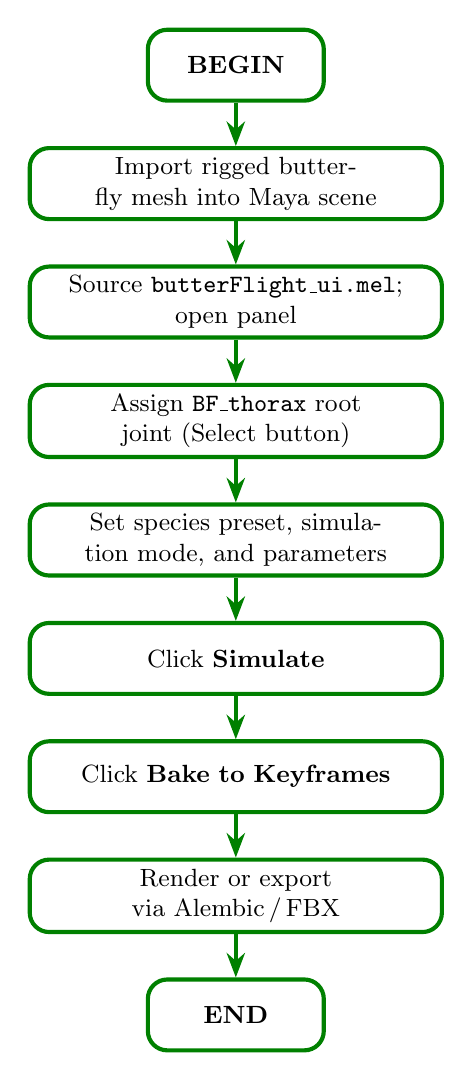
\begin{tikzpicture}[
    node distance=0.55cm,
    proc/.style={
        rectangle, rounded corners=7pt,
        draw=green!50!black, line width=1.5pt,
        text centered, text width=5.0cm,
        minimum height=0.9cm, fill=white, font=\small},
    startstop/.style={
        rectangle, rounded corners=7pt,
        draw=green!50!black, line width=1.5pt,
        text centered, text width=2.0cm,
        minimum height=0.9cm, fill=white,
        font=\small\bfseries},
    dec/.style={
        diamond, aspect=2.6,
        draw=green!50!black, line width=1.5pt,
        text centered, text width=2.8cm,
        inner sep=2pt, fill=white, font=\small},
    arr/.style={->, >=Stealth, line width=1.3pt, color=green!50!black}]

\node[startstop]                    (begin)   {BEGIN};
\node[proc, below=of begin]         (import)  {Import rigged butterfly mesh into Maya scene};
\node[proc, below=of import]        (open)    {Source \texttt{butterFlight\_ui.mel}; open panel};
\node[proc, below=of open]          (assign)  {Assign \texttt{BF\_thorax} root joint (Select button)};
\node[proc, below=of assign]        (params)  {Set species preset, simulation mode, and parameters};
\node[proc, below=of params]        (simulate){Click \textbf{Simulate}};
\node[proc, below=of simulate]      (bake)    {Click \textbf{Bake to Keyframes}};
\node[proc, below=of bake]          (export)  {Render or export via Alembic\,/\,FBX};
\node[startstop, below=of export]   (end)     {END};

% Main vertical flow
\draw[arr] (begin)   -- (import);
\draw[arr] (import)  -- (open);
\draw[arr] (open)    -- (assign);
\draw[arr] (assign)  -- (params);
\draw[arr] (params)  -- (simulate);
\draw[arr] (simulate)-- (bake);
\draw[arr] (bake)    -- (export);
\draw[arr] (export)  -- (end);

\end{tikzpicture}
\caption{ButterFlight workflow. After opening the panel and assigning a rig, the user
  configures species, mode, and simulation parameters, runs the simulation, then
  bakes the result to standard Maya keyframes and optionally triggers an Alembic or
  FBX export.}
\label{fig:workflow}
\end{figure}


\newpage

% ========== Section 2: Authoring Tool Development ==========
\section{Authoring Tool Development}

\subsection{Technical Approach}

\subsubsection{Algorithm Details}

% TODO:
%   - Describe the three main algorithmic modules from Chen et al. 2022:
%       Module 1: Butterfly modeling -- hierarchical skeleton, maneuvering functions,
%                  wing-abdomen interaction (Eq. 1)
%       Module 2: Force computation -- aerodynamic forces (quasi-steady theory, Eq. 4-6)
%                  + curl-noise vortex force (Eq. 7)
%       Module 3: Maneuvering control -- body motion decoupling, velocity computation
%   - List assumptions and simplifications.

\subsubsection{Maya Interface and Integration}

% TODO:
%   - Describe how the algorithms are implemented in the Maya runtime environment.
%   - What is implemented in MEL/Python? (UI panels, parameter sliders, scene setup)
%   - What is implemented in the C++ plug-in? (force simulation, keyframe baking)
%   - Describe relevant Maya objects and data structures (MFnIkJoint, MFnAnimCurve,
%     MFnTransform, MPxCommand, etc.)

\subsubsection{Software Design and Development}

% TODO:
%   - Spec out custom nodes, data structures, and class hierarchies.
%   - Provide a block diagram / flow chart of the program structure.
%   - List third-party software (e.g., Eigen for linear algebra, Maya 2025 API, etc.)

% Placeholder for architecture block diagram:
% \begin{figure}[H]
%   \centering
%   \includegraphics[width=0.9\textwidth]{figures/architecture.png}
%   \caption{ButterFlight software architecture block diagram}
% \end{figure}

\subsection{Target Platforms}

\subsubsection{Hardware}

% TODO: Minimum hardware configuration (processor, RAM, GPU) to run the tool.

\subsubsection{Software}

% TODO: OS version, Maya version, Visual Studio version, SDK versions, etc.

\subsection{Software Versions}

\subsubsection{Alpha Version Features (first prototype)}

% TODO:
%   - List features included in the alpha version.
%   - Describe important development milestones for alpha.
%   - Describe the demo/test scene for alpha.

\subsubsection{Beta Version Features}

% TODO:
%   - List features included in the beta version (adds upon alpha).
%   - Describe important development milestones for beta.
%   - Describe the demo/test scene for beta.

\subsubsection{Description of Demos and Tutorials}

% TODO:
%   - How will users learn to use the tool?
%   - Describe demos and/or tutorials shipping with the final version.

\newpage

% ========== Section 3: Work Plan ==========
\section{Work Plan}

\subsection{Tasks and Subtasks}

% TODO: List and number all tasks and subtasks.
% Each main task must have at least 3 subtasks.
% For each task: name, duration, description, assigned team member(s).
% Use the format below for each task:
%
% \textbf{Task 1 --- Task Name}\\
% \textbf{Duration:} X weeks\\
% Description (at least 3 sentences).
%
% \begin{itemize}
%   \item \textbf{Subtask 1.1 --- Name}: Description (2--3 sentences).
%   \item \textbf{Subtask 1.2 --- Name}: Description.
%   \item \textbf{Subtask 1.3 --- Name}: Description.
% \end{itemize}

% Suggested task breakdown:
%   Task 1: Environment Setup and Maya Plugin Scaffolding
%   Task 2: Butterfly Skeleton Rig and Maneuvering Functions
%   Task 3: Aerodynamic Force Model
%   Task 4: Curl-Noise Vortex Force
%   Task 5: Maneuvering Control and Body Motion Decoupling
%   Task 6: MEL/Python UI Panel
%   Task 7: Single Butterfly Path Following Demo
%   Task 8: Swarm Simulation and Aggregation
%   Task 9: Export (Alembic / FBX) and Final Integration
%   Task 10: Testing, Debugging, and Demo Scenes

\subsection{Milestones}

\subsubsection{Alpha Version}

% TODO: List tasks and subtasks that must be completed for the alpha version.

\subsubsection{Beta Version}

% TODO: List tasks and subtasks that must be completed for the beta version.

\subsection{Schedule}

% TODO: Insert Gantt chart showing all tasks, durations, and milestone dates
% (alpha: Mar 25, beta: Apr 15, final demo: May 5, code due: May 11).

% Placeholder for Gantt chart:
% \begin{figure}[H]
%   \centering
%   \includegraphics[width=\textwidth]{figures/gantt.png}
%   \caption{ButterFlight project schedule}
% \end{figure}

\newpage

% ========== Section 4: Related Research ==========
\section{Related Research}

% The Related Research section is fulfilled by including the Literature Survey.
% Insert the content of Literature_Survey_ButterFlight.tex here,
% or \input it directly:
%
% \input{../Literature_Survey/Literature_Survey_ButterFlight_content.tex}

% TODO: Paste or \input the full Literature Survey content (introduction,
% research evolution graph, paper descriptions, and references).

\newpage

% ========== Bibliography ==========
\begin{thebibliography}{99}

\bibitem{Chen2022}
CHEN Q., LU T., TONG Y., LUO G., JIN X., DENG Z.:
A Practical Model for Realistic Butterfly Flight Simulation.
\textit{ACM Transactions on Graphics (TOG)} 1, 1 (2022), 12 pages.

\bibitem{Ellington1984a}
ELLINGTON C.~P.:
The aerodynamics of hovering insect flight. I. The quasi-steady analysis.
\textit{Philosophical Transactions of the Royal Society of London. B,
Biological Sciences} 305, 1122 (1984), 1--15.

\bibitem{Ellington1984b}
ELLINGTON C.~P.:
The aerodynamics of hovering insect flight. V. A vortex theory.
\textit{Philosophical Transactions of the Royal Society of London. B,
Biological Sciences} 305, 1122 (1984), 115--144.

\bibitem{Reynolds1987}
REYNOLDS C.~W.:
Flocks, herds and schools: A distributed behavioral model.
In \textit{Proceedings of the 14th Annual Conference on Computer Graphics
and Interactive Techniques} (1987), pp.~25--34.

\bibitem{BettsWootton1988}
BETTS C.~R., WOOTTON R.~J.:
Wing shape and flight behaviour in butterflies (Lepidoptera: Papilionoidea
and Hesperioidea): a preliminary analysis.
\textit{Journal of Experimental Biology} 138, 1 (1988), 271--288.

\bibitem{Perlin2002}
PERLIN K.:
Improving noise.
In \textit{ACM Transactions on Graphics (TOG)}, Vol.~21.
ACM, 2002, pp.~681--682.

\bibitem{WuPopovic2003}
WU J., POPOVI\'C Z.:
Realistic modeling of bird flight animations.
\textit{ACM Transactions on Graphics (TOG)} 22, 3 (2003), 888--895.

\bibitem{Bridson2007}
BRIDSON R., HOURIHAM J., NORDENSTAM M.:
Curl-noise for procedural fluid flow.
\textit{ACM Transactions on Graphics (TOG)} 26, 3 (2007), 46--es.

\bibitem{WilsonAlbertani2014}
WILSON T., ALBERTANI R.:
Wing-flapping and abdomen actuation optimization for hovering in the
butterfly \textit{Idea leuconoe}.
In \textit{52nd Aerospace Sciences Meeting} (2014), 0009.

\bibitem{Wang2014}
WANG X., JIN X., DENG Z., ZHOU L.:
Inherent noise-aware insect swarm simulation.
In \textit{Computer Graphics Forum}, Vol.~33.
Wiley Online Library, 2014, pp.~51--62.

\bibitem{Wang2015}
WANG X., REN J., JIN X., MANOCHA D.:
BSwarm: biologically-plausible dynamics model of insect swarms.
\textit{Proceedings of the 14th ACM SIGGRAPH/Eurographics Symposium on
Computer Animation} (2015), 111--118.

\bibitem{Sridhar2016}
SRIDHAR M., KANG C.-K., LANDRUM D.~B.:
Instantaneous lift and motion characteristics of butterflies in free flight.
In \textit{46th AIAA Fluid Dynamics Conference} (2016), 3252.

\bibitem{Chen2019}
CHEN Q., LUO G., TONG Y., JIN X., DENG Z.:
Shape-constrained flying insects animation.
\textit{Computer Animation and Virtual Worlds} 30, 3--4 (2019), e1902.

\bibitem{Sridhar2020}
SRIDHAR M., KANG C.-K., LEE T.:
Geometric formulation for the dynamics of monarch butterfly with the effects
of abdomen undulation.
In \textit{AIAA Scitech 2020 Forum} (2020), 1962.

\bibitem{Will2020}
WILL H.:
Dynamic Bone.
Unity Asset Store, 2020.
\url{https://assetstore.unity.com/packages/tools/animation/dynamic-bone-16743}.

\end{thebibliography}

\end{document}
